\section{Nuclio}
\label{sec:nuclio}

%%%%
\subsection{A Customizable Serverless Platform}
\label{sec:nuclio-introduction}
To better understand the following subsections and the language they contain, we begin with a basic overview of Nuclio as our framework. Nuclio is an open-source serverless platform designed for data-intensive, compute-intensive workloads. Unlike widely known cloud-based solutions such as AWS Lambda\footnote{\url{https://aws.amazon.com/de/lambda/}} or Google Cloud Functions\footnote{\url{https://cloud.google.com/functions}}, Nuclio offers the flexibility to deploy serverless functions directly on your own infrastructure on an open source basis. This allows for greater control and customisation and opens up possibilities that might be limited on vendor-bound platforms.
The open source nature of Nuclio allows us to optimize the platform based on specific project requirements and to experiment flexibly with new concepts to improve performance and cost metrics. This adaptability led our project manager, Trevor Schirmer, to select Nuclio for our work and further developments.

\subsection{Architecture components}
\label{sec:nuclio-components}
Nuclio's architecture includes several key components: Trigger, Processor, Worker, Controller, Builder, Dashboard and Scaler. Triggers, activated by event sources, initiate actions that are handled by processors. They can be divided into the following event classes\footnote{\url{https://nuclio.io/latest/concepts/architecture/}}:
\begin{itemize}
    \item Synchronous request/response - the client makes a request and waits for an immediate response, e.g. HTTP
    \item Asynchronous message queue request - messages are distributed to the subscribers, e.g. RabbitMQ\footnote{\url{https://www.rabbitmq.com/}}
    \item Message or record streams - an ordered set of messages or record updates are handled sequentially, e.g.  Kafka\footnote{\url{https://kafka.apache.org/}}
    \item Record or Data Polling - a filtered set of data objects is retrieved from an external data source or database, e.g.  DynamoDB\footnote{\url{https://aws.amazon.com/de/dynamodb/}}
\end{itemize} 
This project report is limited to the HTTP-based request-reply trigger, which was already used intensively in previous work by Schirmer et al. \cite{schirmer2023profaastinate}.
A processor listens for one or more of the triggers and executes user functions with one or more parallel workers\footnote{\url{https://nuclio.io/latest/introduction/}}. 
The workers use language-specific runtimes to execute the function; a distinction is made between the types:
\begin{itemize}
    \item Native - real-time routines based on Golang or C.
    \item SHMEM - the processor communicates with the SHMEM function runtime via zero-copy shared memory channels, e.g. Python
    \item Shell - for command line execution functions or executable binary files\footnote{\url{https://nuclio.io/latest/concepts/architecture/}}.
\end{itemize}
\vspace{5mm} 
\begin{figure}
    \centering
    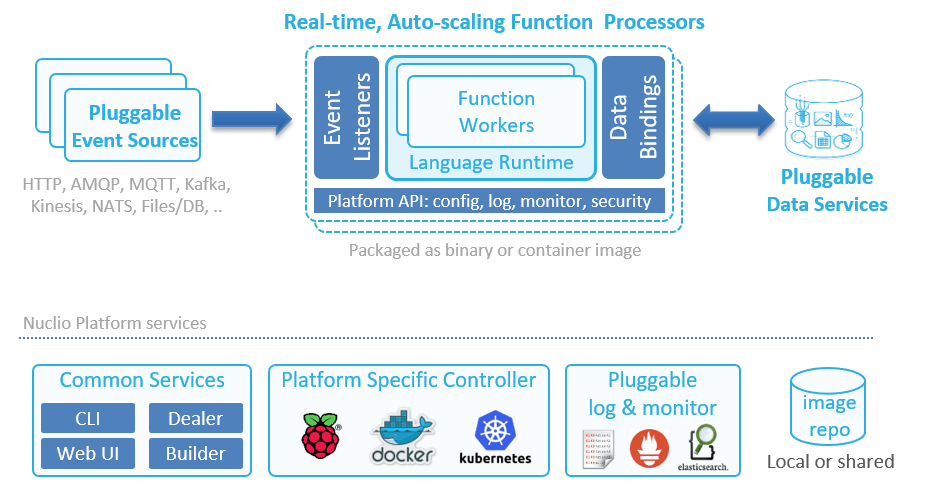
\includegraphics[width=0.48\textwidth]{figures/profaastinate/nuclio-architecture.png} % Adjust the width as needed
    \caption{
         Nuclio's high-level architecture\protect\footnote{\url{https://nuclio.io/latest/introduction/}}.
    }
    \label{fig:nuclio-architecture}
\end{figure}

The dashboard is a standalone microservice that is accessed via HTTP and contains a code editor GUI. The user can access this or alternatively the nuclio CLI to provide function code via the function registry. However, in order to be able to execute the function in the worker, the builder is required, which builds a binary file or a container image from raw code and optional build instructions and dependencies, which is pushed to an image repository\footnote{\url{https://nuclio.io/latest/introduction/}}.

In this work, the dashboard was mainly used to write the function code, working only with a local registry, primarily using a Native and SHMEN worker for Go and Python. 

\begin{figure}
    \centering
    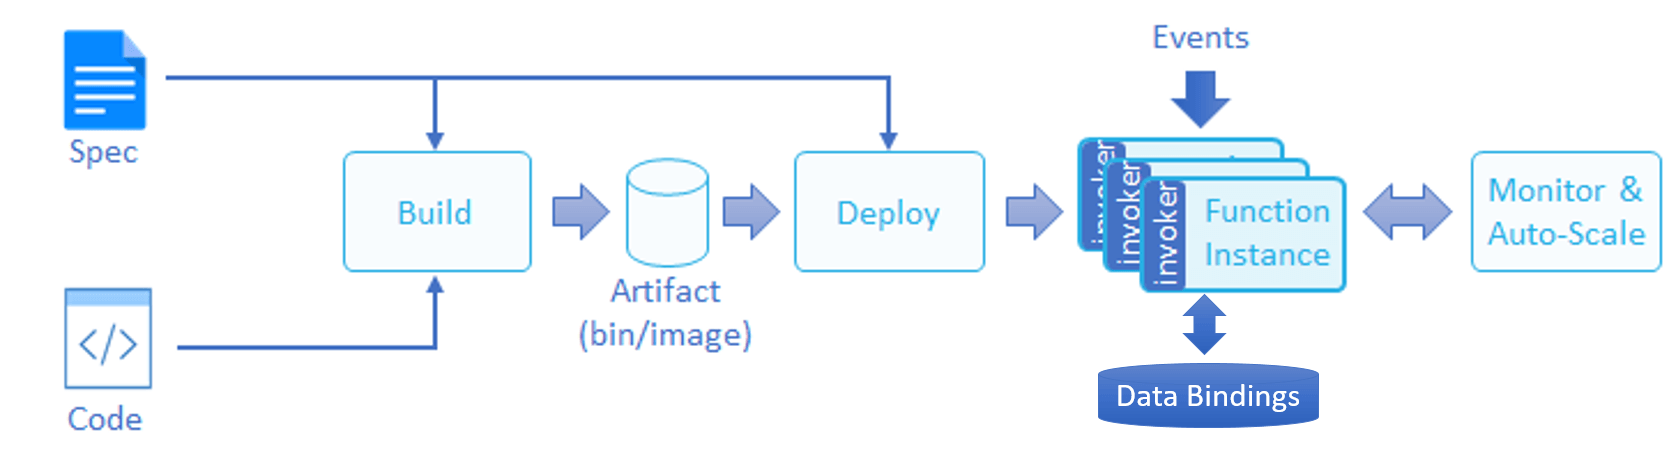
\includegraphics[width=0.48\textwidth]{figures/profaastinate/nuclio-build-deploy.png} 
    \caption{
         Function build and deployment flow\protect\footnote{\url{https://nuclio.io/latest/concepts/architecture/}}.
    }
    \label{fig:nuclio-build-deploy}
\end{figure}

A controller then connects the various components by receiving the specifications of functions and event sources. It invokes builders and processors via an orchestration platform and manages function elasticity, lifecycle and versions.

\label{sec:nuclio-namespace}
All the resources, such as functions or triggers, that are described earlier, can then be logically grouped or isolated in a Nuclio Namespace. This enables better control of user access and authorization. 

The Nuclio system as a whole can then be run in different environments, either as standalone Docker containers or on container orchestration tools like Kubernetes. Our research focused mainly on the Docker and Minikube container environments. The latter is a local cluster\footnote{\url{https://minikube.sigs.k8s.io/}} of the orchestration platform Kubernetes\footnote{\url{https://kubernetes.io/}}. 

Finally, it's worth noting that certain Nuclio features, such as "scale to zero", are exclusively accessible in on-premises environment of Iguazio's Nuclio Enterprise Edition, facilitating efficient function execution\footnote{\url{https://www.iguazio.com/}}.